\begin{frame}{Functional sensitivity}
Let $p_0(\nu_k)$ be the original Beta prior on sticks.

Suppose we wish to replace $p_0$ with another distribution $p_1$. Define the ``contaminated" prior as:
\begin{align*}
p_c(\nu_k \vert \epsilon) \propto
p_{0}(\nu_k)\exp(\epsilon\phi(\nu_k))
\end{align*}
where $\phi(\nu_k) = \log p_1(\nu_k) - \log p_0(\nu_k)$.

\begin{figure}[!h]
\centering
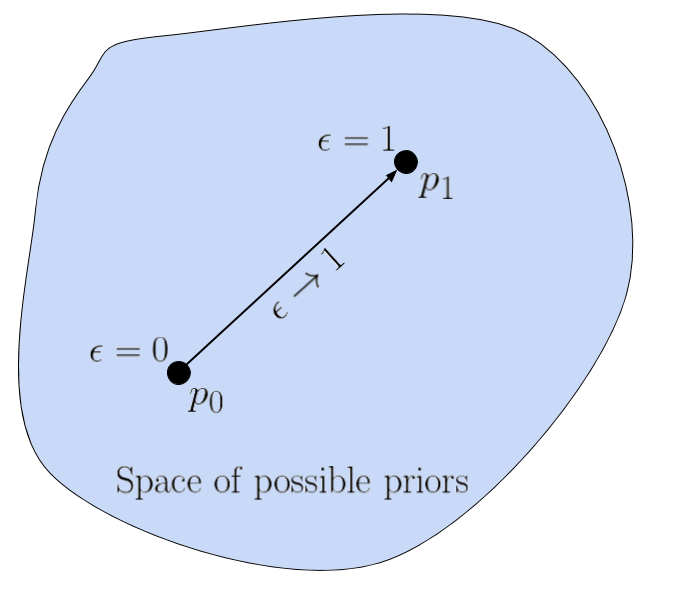
\includegraphics[width = 0.45\textwidth]{./figures/static_figures/functional_perturbation.png}
\setlength{\textfloatsep}{-10pt}
\end{figure}

\end{frame}

\begin{frame}{Functional sensitivity: influence functions}

Consider a posterior statistic of interest $g(\eta)$, e.g.
\begin{align*}
g_{\textrm{cl}}(\eta) = \Expect_{q_{\eta}} \left[ \#\text{clusters} \right]
\end{align*}

Let $S_g$ be the \textit{local sensitivity} of $g$ with respect to a hyper-parameter $\epsilon$
\begin{align*}
S_g := \frac{d}{d\epsilon} \; g(\eta(\epsilon))
\end{align*}

\pause

The local sensitivity can be expressed as an inner-product between an \textit{influence function} $\Psi$
and the functional perturbation $\phi$ in an appropriate Hilbert space:
\begin{align*}
S_g &= \langle \Psi, \phi\rangle \\
&= \int \Psi(\nu) \phi(\nu) p_0(\nu) \;d\nu
\end{align*}


\end{frame}

\begin{frame}{Iris data: influence functions}
  \begin{figure}[!h]
    \centering
    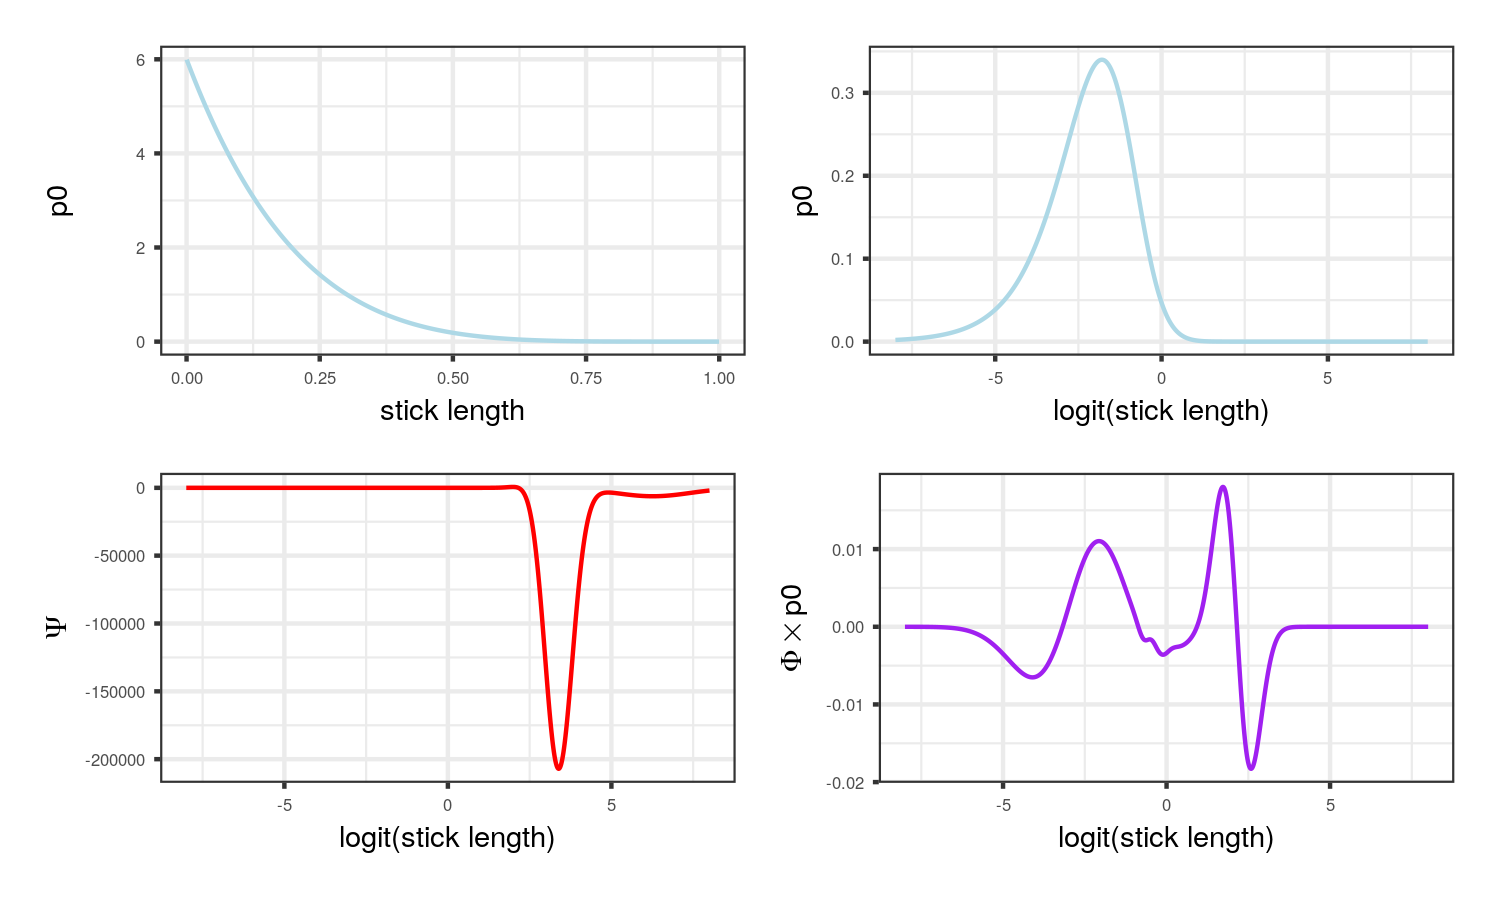
\includegraphics[width = \textwidth]{./figures/iris_influence_function.png}
    \caption*{The influence function for the number of clusters, $g_{\textrm{cl}}$.}
\end{figure}
\end{frame}

\begin{frame}{Iris data: functional perturbations}
\begin{figure}[!h]
    \centering
    \only<1>{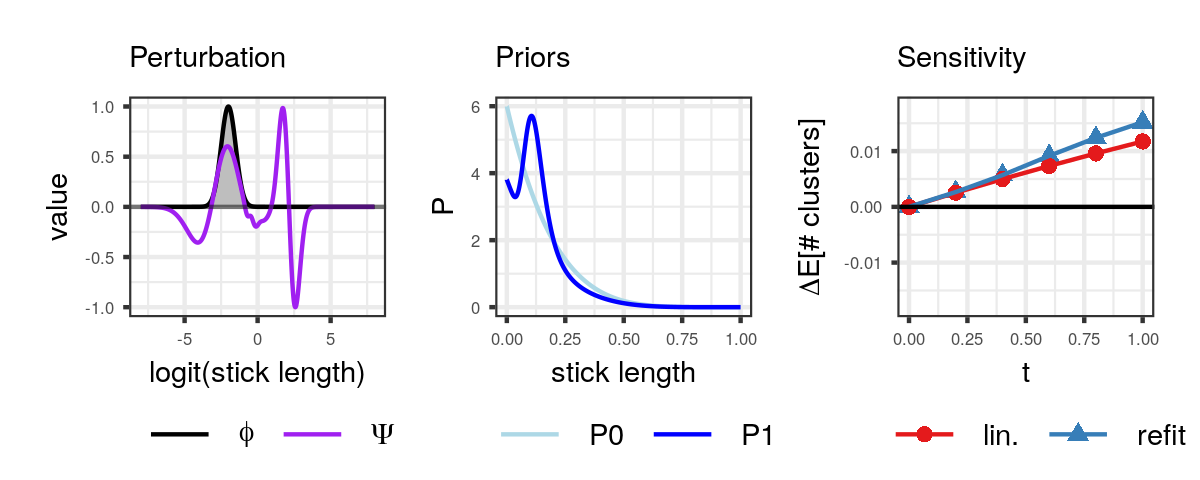
\includegraphics[width = 0.8\textwidth]{./figures/iris_func_sens0.png}}
    \only<2>{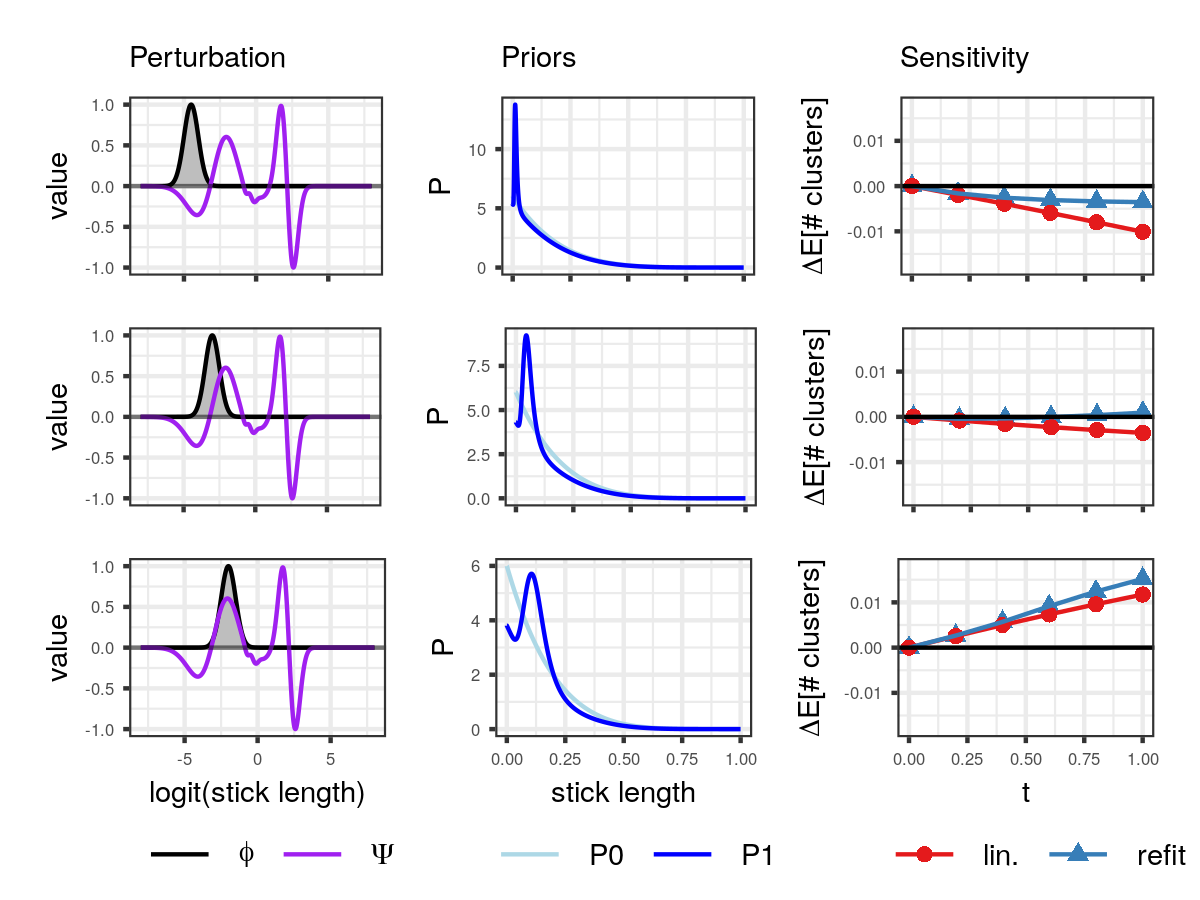
\includegraphics[width = 0.8\textwidth]{./figures/iris_func_sens1.png}}
\end{figure}
\end{frame}

\begin{frame}{Functional perturbations: worst-case}

There are many possible choices for $p_1$.

Given a posterior quantity $g$,
we can find the {\itshape worst-case} perturbation in a ball of
radius $\delta$, that is, find the direction such that
$|S_g|$ is maximized.

\vspace{-1em}

\begin{figure}[!h]
\centering
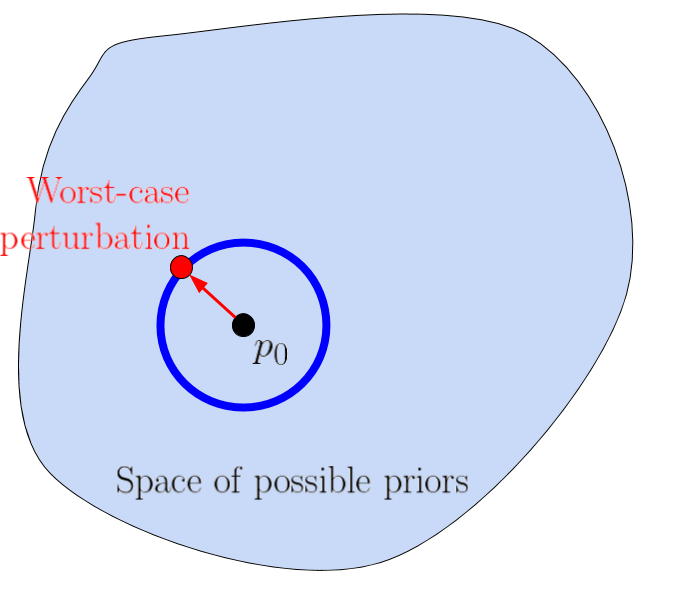
\includegraphics[width = 0.4\textwidth]{./figures/static_figures/functional_perturbation_worst_case.png}
\setlength{\textfloatsep}{-10pt}
\end{figure}

\vspace{-1em}

Specifically, we consider the L-infinity ball of radius $\delta$:
\begin{align*}
  B_\delta := \{\phi : \|\phi\|_\infty < \delta\}
\end{align*}

\end{frame}

\begin{frame}{Iris data: worst-case perturbation}
  \begin{figure}[!h]
    \centering
    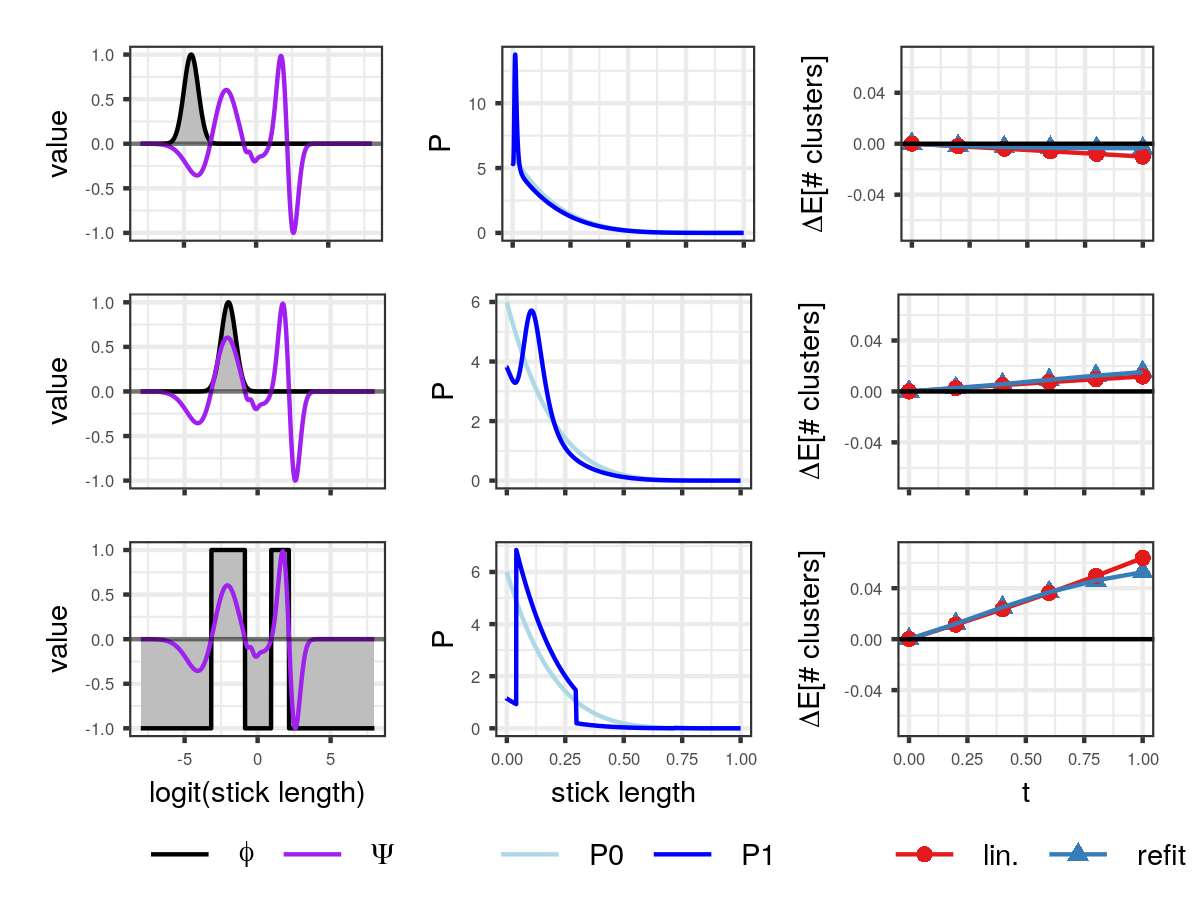
\includegraphics[width = 0.8\textwidth]{./figures/iris_worst_case.png}
\end{figure}
\end{frame}
